\chapter{Tribler's current state}

Tribler's IO has been a problem for years \cite{pouwelse2014reduce}.
In May 2013 Tribler read and wrote 660 Megabytes per hour to and from disk.
Back in April 2014 this number was somewhat reduced to 623.
In May 2014 efforts were made to reduce this enormous amount of IO and after batching several database statements the number further dropped to 538 Megabytes per hour.

As performing IO operations blocks a thread (see Chapter X \todo{Write a chapter about the treading model in python and reference to it.}), it is essential keep track of this information and to work towards reducing this number.
So far this metric has only been measured sporadically by hand, running Tribler for an arbitrarily amount of time and check the amount of IO by using iotop\footnote{\url{http://guichaz.free.fr/iotop/}}.
This produces an overview similar to Figure \ref{fig:iotop_tribler_april_2014}.
Since 2014 no work or measurements have been done related to this issue.

\begin{figure}[h]
	\makebox[\textwidth][c]{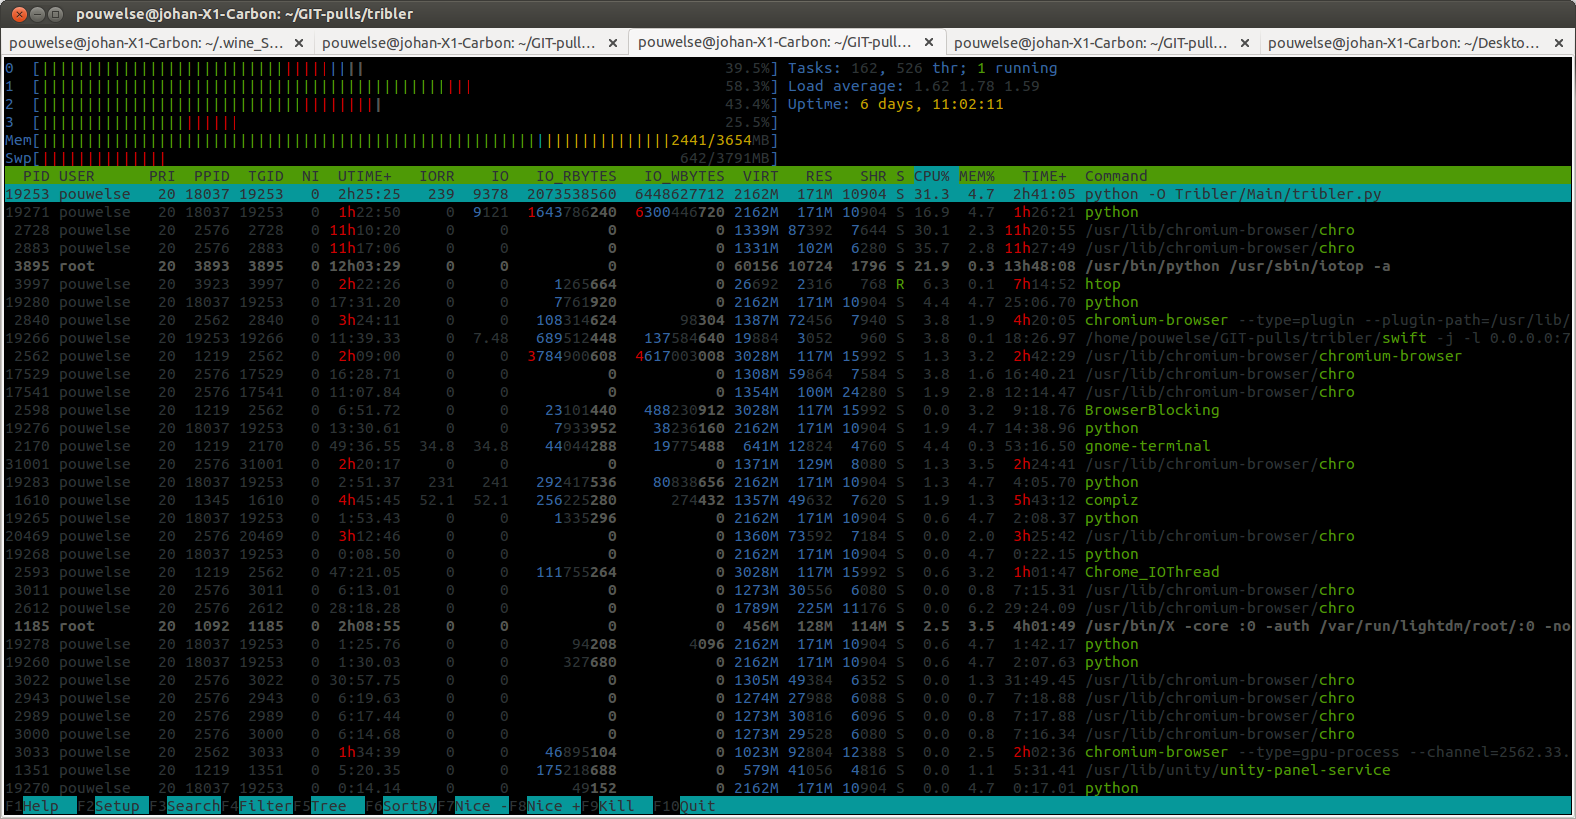
\includegraphics[width=0.95\paperwidth]{iointribler/images/iotop}}
	\caption{A screenshot of iotop showing Tribler's IO, from Johan Pouwelse \cite{pouwelse2014reduce}.}
	\label{fig:iotop_tribler_april_2014}
\end{figure}

In the meantime, Tribler has seen several changes to its code base including the addition of the MultiChain: Tribler's own Blockchain like structure \cite{norberhuis2015multichain}.
This feature heavily relies on its database to store blocks and other information about the user and other peers their chains.
Moreover, the MultiChain makes use of its own database rather than Dispersy's.
Norberhuis points out: ``The information is stored in two places within Tribler and this could be eliminated. It would reduce the disk footprint and the amount of read/write transactions as only one database would have to be maintained. The I/O ineractions are a problem according to Tribler maintainers.'' \cite{norberhuis2015multichain}, yet numbers on how much IO the MultiChain generates are not presented.
This makes it hard to estimate Tribler's current IO rates.
 
Furthermore, a feature called ``credit mining'' is currently in development that will also interact with the database of Tribler.
There are no metrics on the current situation of Tribler and it's hard if not impossible to estimate the impact of any addition to come.

To observe the current situation, we have measured Tribler running idle (i.e. no human interaction) for X hours.
For this experiment we run Tribler version 6.6.0-pre-exp which is a pre-release of 6.6, because it includes the MultiChain code.
The hardware used during this experiment can be seen in Table \ref{table:tribler_idle}.

\begin{table}[h]
	\centering
	\begin{tabular}{l|l}
Hardware	& Specifications \\ \hline
CPU			&  \\ 
HDD			&  \\ 
RAM			&  \\
	\end{tabular}
	\caption{Hardware used during the idle iotop measurement of Tribler 6.6.0-pre-exp.}
	\label{table:tribler_idle}
\end{table}

The results are visible in Figure X.
From these results we observe that Tribler current has an IO of Y.
To observe the individual components separately, we have created a breakdown the database queries performed by Tribler.
This breakdown is visible in Table Z.
As we can see, B is doing the most IO... \todo{Fill in the stuff when experiment done}

